\pdfminorversion=4
\documentclass{beamer}
\usepackage[utf8]{inputenc}

\usepackage[
backend=biber,
style=alphabetic,
sorting=ynt
]{biblatex}
 
\addbibresource{bibliography.bib}

\usepackage{textcomp}
\usepackage[T1]{fontenc}
\usepackage{multirow}
\usepackage{float}
\usepackage[caption = false]{subfig}
\usepackage{longtable}
\usepackage{listings}
\usepackage{mathtools}
\DeclareMathOperator{\tr}{Tr}
\usepackage{commath}
\usepackage{bbold}
\usepackage{xcolor}
\usepackage{physics}
%\usepackage[margin=1.8cm]{geometry}

\usepackage{tikz-cd} 
\usepackage{amsmath}
\usepackage{amsfonts}
\usepackage{amssymb}
\usepackage{amsthm}
\usepackage{graphicx}
\usepackage[colorinlistoftodos]{todonotes}
\usepackage[colorlinks=true, allcolors=blue]{hyperref}
\usepackage{siunitx}
\sisetup{separate-uncertainty=true}

\usepackage[sc]{mathpazo}
\linespread{1.05}         % Palladio needs more leading (space between lines)
\usepackage[T1]{fontenc}

\newcommand{\diag}[1]{\text{diag}\qty(#1)}
\newcommand{\Lagr}{\mathcal{L}}
\newcommand{\const}{\text{const}}
\newcommand{\sign}[1]{\text{sign}\qty(#1)}
\usetheme{Rochester}

\title{Relativistic Non-Ideal Flows}
\author{Jacopo Tissino}
\date{24/09/2019}

\begin{document}

\frame{\titlepage}

\begin{frame}
    \frametitle{The Schwarzschild metric}
    Flat metric:

    \begin{equation*}
        \dd{s}^2 = -\dd{t}^2 + \dd{r}^2 + r^2 \qty(\dd{\theta}^2 + \sin^2\theta \dd{\varphi})\,.
    \end{equation*}

    Schwarzschild metric:

    \begin{equation*}
        \dd{s}^2 = -\qty(1-\frac{2M}{r})\dd{t}^2 + \frac{1}{1-\frac{2M}{r}} \dd{r}^2
        + r^2 \qty(\dd{\theta}^2 + \sin^2\theta \dd{\varphi})\,,
    \end{equation*}
    %
    where \(c = G = 1\).

    % The radial coordinate \(r\) can be defined with the 2-sphere's area: \(A \overset{!}{=} 4 \pi r^2\) since the angular metric is flat.

    % The singularity at \(r = 2M \) is not physical: there are other coordinates in which it disappears and the physical behaviour is revealed, objects \emph{can} actually reach the horizon in finite time.
\end{frame}

\begin{frame}
    \frametitle{The Schwarzschild metric}
    \begin{figure}
        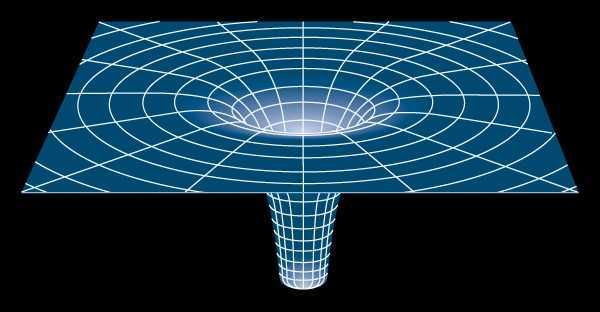
\includegraphics[width=\textwidth]{figures/Schwarzschild-Space}
    \end{figure}

    % Circles are spaced further apart on the manifold than their radii's difference
\end{frame}

\begin{frame}
    \frametitle{The stress-energy tensor}

    The component \(T^{\mu\nu}\) is the flux of \(\mu\)-th component of the four-momentum \(p^\mu\) through a surface of constant coordinate \(x^\nu\).

    For an ideal fluid (\(\eta = \xi = \kappa = 0\)) in the Local Rest Frame:

    \begin{equation*}
        T^{\mu\nu} =
        \begin{bmatrix}
        \rho   &   &   &  \\
           & p  &   &  \\
           &   & p  &  \\
           &   &   & p
       \end{bmatrix}_{\text{fid}} \,.
    \end{equation*}
\end{frame}

\begin{frame}
    \frametitle{The Local Rest Frame}

    A set of vectors \(V^\mu _{(\alpha)}\)  such that
    %
    \begin{equation*}
        g_{\mu\nu} V^\mu _{(\alpha)} V^\nu _{(\beta)} = \eta_{(\alpha) (\beta)}\,.
    \end{equation*}
\end{frame}

\begin{frame}
    \frametitle{The PSTF moments}
\end{frame}

\end{document}
